\documentclass[document.tex]{subfiles} 

\begin{document}

\chapter{إقلاع الحاسب ومحمل النظام \en{Bootloader}}
أحد أهم الأساسيات في برمجة نظام تشغيل هي كتابة محملٌ له ، هذا المحمل يعمل على نسخ نواة النظام من أحد الأقراص الى الذاكرة الرئيسية ثم ينقل التنفيذ الى النواة ، وهكذا تنتهي دورة عمل المحمل ويبدأ نظام التشغيل متمثلا في النواة بالبدء بتنفيذ الاوامر والمهمات وتلبية إحتياجات المستخدم. في هذا الفصل سندرس كيفية برمجة المحمل وماهيته وسيتم الاقلاع من قرص مرن بنظام \en{FAT12} ، فالغرض هذه المرحلة هو دراسة أساسيات المحمل وتحميل وتنفيذ نواة مبسطة .

\section{إقلاع الحاسب}

إقلاع الحاسب (\en{Boot-Strapping}) هي أول خطوة يقوم بها الجهاز عند وصله بالكهرباء لتحميل نظام التشغيل، وتبدأ هذه العملية مباشرة عند الضغط على مفتاح التشغيل في الحاسب ، حيث ترسل إشارة كهربائية\footnote{هذه الإشارة تحوي على بت ( \en{bit} ) تدل قيمته اذا كانت \en{1} على أنه تم تشغيل الحاسب.} الى اللوحة الام ( \en{MotherBoard} ) والتي تقوم بتوجيهها الى وحدة موزد الطاقة (\en{Power Supply Unit}). بعد ذلك يأتي دور وحدة \en{PSU} لكي تقوم بمهمة تزويد الحاسب وملحقاته بالكمية المطلوبة من الطاقة، وإرسال اشارة \en{Power Good} إلى اللوحة الام وبالتحديد الى نظام ال \en{BIOS} .
تدل هذه الاشارة على أنه تم تزويد الطاقة الكافية ، وفورا سيبدأ برنامج الفحص الذاتي ( \en{Power on Self Test} ) الذي يعرف اختصاراً ب \en{POST} بفحص أجهزة ومحلقات الحاسب (مثل الذاكرة ولوحة المفاتيح والماوس والناقل التسلسلي ...الخ) والتأكد من أنها سليمة.
بعدها يقوم ال \en{POST} بنقل التحكم الى نظام ال \en{BIOS} حيث سيقوم ال \en{POST} بتحميل ال \en{BIOS} الى نهاية الذاكرة \en{0xFFFF0} و سيقوم أيضا بوضع تعليمة قفز ( \en{jump} ) في أول عنوان في الذاكرة الى نهاية الذاكرة ، كذلك من مهام ال \en{POST} هي تصفير المسجلين \en{CS:IP} وهذا يعني أن أول تعليمية سينفذها المعالج هي تعليمة القفز الى نهاية الذاكرة وبالتحديد الى ال \en{BIOS} .
يستلم ال \en{BIOS} التحكم ويبدأ في انشاء جدول المقاطعات ( \en{Interrupt Vector Table} ) وتوفير العديد من المقاطعات ،ويقوم بالمزيد من عمليات الفحص والاختبار للحاسب ، وبعد ذلك يبدأ في مهمة البحث عن نظام تشغيل في الاجهزة الموجودة بناءا على ترتيبها في اعدادات ال \en{BIOS} في برنامج \en{Setup} ،وفي حالة لم يجد ال \en{BIOS} جهازا قابلا للاقلاع في كل القائمة فانه يصدر رسالة خطأ بعدم توفر نظام تشغيل ويوقف الحاسب عن العمل ( \en{Halt} ) ، وفي حالة توفر جهازاً قابلاً للإقلاع سيقوم ال \en{BIOS} بتحميل القطاع الأول منه ( يحوي هذا القطاع على برنامج المحمل) الى الذاكرة الرئيسية وبالتحديد الى العنوان الفيزيائي \en{0x07c00} وسيُنقَل التنفيذ الى المحمل.\\

خلال هذه المهمة (اقلاع النظام) يوفر لنا نظام ال \en{BIOS} العديد من المقاطعات على جدول المقاطعات والذي يتم انشائه بدءاً من العنوان \en{0x0} ، هذه المقاطعات هي خدمات يوفرها لنا نظام البايوس لاداء وظيفة معينة مثل مقاطعة لطباعة حرف على الشاشة.
واحدة من أهم المقاطعات التي يستخدمها نظام البايوس للبحث عن جهاز الاقلاع هي المقاطعة \en{int 0x19} حيث تكمن وظيفتها في البحث عن هذا الجهاز ومن ثم تحميل القطاع الأول منه الى العنوان الفيزيائي \en{0x07c00} ونقل التنفيذ اليه . طريقة البحث والتحميل ليست بالامر المعقد حيث على هذه المقاطعة البحث في أول قطاع (من أي جهاز موجود على قائمة الاجهزة القابلة للاقلاع) عن التوقيع \en{0xAA55} وهي عبارة عن بايتين يجب أن تكون على آخر القطاع الاول  تدل على أن هذا الجهاز قابل للاقلاع.
ومن الجدير بالذكر أن المقاطعات التي يوفرها لنا نظام البايوس يمكن استخدامها فقط اذا كان المعالج يعمل في النمط الحقيقي \en{Real Mode} أما إذا تم تغيير نمط المعالج الى النمط المحمي \en{Protected Mode} - كما سنرى ذلك لاحقا- فانه لن يمكن الاستفادة من هذه المقاطعات بل سيتسبب استخدامها في حدوث استثناءات ( \en{Exception} ) توقف عمل الحاسب.

\section{محمل النظام \en{Bootloader}}
محمل النظام هو برنامج وظيفته الرئيسية هي تحميل نواة نظام التشغيل ونقل التنفيذ اليها.هذا المحمل يجب ان تتوفر فيه الشروط الاتية :

\begin{enumerate}
\item حجم البرنامج يجب أن يكون \en{512} بايت بالضبط.
\item أن يتواجد على القطاع الأول في القرص : القطاع رقم \en{1} ، الرأس \en{0} ، المسار \en{0} ، وأن يحمل التوقيع المعروف.
\item أن يحوي شفرة تحميل النواة ونقل التنفيذ اليها.
\item أن يكون البرنامج \en{object code} خالي من أي أضافات ( \en{header,symbol table,...etc} ) وهو ما يعرف أيضا بـ \en{ Flat Binary} .

\end{enumerate}

الشرط الأول يُّقيد وظيفة المحمل وقدرته على توفير خصائص متقدمة\footnote{مثل خاصية ال \en{Safe Mode} }، حيث أن هذا الحجم لا يكفي لكي يبحث المحمل عن نواة النظام وتمهيد الطريق لها للبدء بتنفيذها ، وبسبب أن النواة ستكون \en{32-bit} فانه يجب تجهيز العديد من الأشياء بدءاً من جداول الواصفات (العامة والخاصة) وتفعيل البوابة \en{A20} وانتهاءاً بتغيير نمط المعالج الى النمط المحمي والقفز الى النواة للمباشرة في تنفيذها . كل ذلك يحتاج الى حجم أكبر من الحجم المشروط لذلك عادة ما يلجأ مبرمجوا المحملات الى تجزئيها على مرحلتين وهو ما يسمى ب \en{Multi-Stage Boot Loader} .
الشرط الثاني للمحمل وهو أن يتواجد على أول قطاع في القرص وهو يحمل العنوان الفيزيائي التالي:
\begin{itemize}
\item القطاع رقم \en{1}
\item المسار رقم \en{0}
\item الرأس رقم \en{0}
\end{itemize}

وتحقيقُ هذا الشرط ليس بالأمر المعقد خصوصا مع توفر العديد من الادوات التي تساعد على نسخ مقطع من قرص ما الى مقطع في قرص آخر ، أما الشق الثاني من الشرط فهو متعلق بتمييز القطاع الاول كقطاع قابل للاقلاع من غيره ، حيث حتى يكون القطاع قابلا للاقلاع فانه يجب أن يحمل التوقيع \en{0xAA55} في البايت رقم \en{510} و \en{511} . وبدون هذا التوقيع فان البايوس (وتحديدا مقاطعة رقم \en{0x19}) لن تتعرف على هذا القطاع كقطاع قابلٌ للإقلاع.
أما الشرط الثالث فهو شرط اختياري وليس اجباري ، فمن الممكن أن تكون وظيفة المحمل هي عرض رسالة ترحيب فقط ! ولكن في أغلب الحالات الواقعية يجب أن تُحمَّل النواة  وتُنفَّذ عن طريق هذا المحمل. وقد أسلفنا وذكرنا أن تحميل نواة \en{32-bit} يختلف عن تحميل نواة \en{16-bit} ، حيث في الاولى يجب تجهيز الطريق أمام النواة وتفعيل بعض الخصائص لذلك وَجب تقسيم مهمة محمل النظام الى مرحليتن - كماسنرى ذلك - ، أما في حالة كانت النواة \en{16-bit} فانه يمكن تحميلها بمرحلة واحدة فقط .
والشرط الاخير يتعلق بصيغة الملف التنفيذي للمحمل، حيث أغلب المترجمات تخرج صيغ تنفيذية تحوي على الكثير من المعلومات المضافة من قبله ( كصيغ \en{ELF,PE,COFF,...etc} ) وهذا ما يجعل عملية تنفيذ المحمل وتشغيله من قبل البايوس مستحيلة ، فالبايوس عندما يقرأ محمل النظام الى الذاكرة فانه ينقل التنفيذ الى أول بايت فيه والذي يجب ان يكون قابل للتنفيذ وليس معلومات أو هيدر عن الملف - كما في حالة الصيغ السابق ذكرها- . لذلك يجب أن تكون صيغة المحمل هي عبارة عن الصيغة الثنائية المقابلة للأوامر الموجودة فيه بدون أي اضافات أي \en{Object Code} او  \en{Flat Binary}.\\

ويجدر بنا الحديث عن لغة برمجة محمِّل النظام، فغالبا تستخدم لغة التجميع (\en{Assembly 16-bit}) لأسباب كثيرة ، منها أن الحاسب عندما يبدأ العمل فان المعالج يكون في النمط الحقيقي تحقيقا لأغراض التوفقية ( \en{Backward Compatibility} ) مع الأجهزة السابقة ، أيضا استخدام لغة التجميع  \en{16-bit} يجعل من الممكن استدعاء مقاطعات وخدمات البايوس - قبل الانتقال الى بيئة \en{32-bit} - ، أخيراً  لا حاجة لملفات وقت التشغيل \en{run-time library} ، حيث أن لغة التجميع ماهي الا مختصرات للغة الآلة \en{Machine Language}.
كل هذا لا يجعل عملية كتابة محمِّل النظام بلغة السي مستحيلا ! فهناك كمٌّ كبير من المحملات تستخدم لغة السي والتجميع في آن واحد ( مثل \en{GRUB,NTLDR,LILO...etc} ) ، لكن قبل برمجة مثل هذه المحملات يجب برمجة بعض ملفات ال \en{run-time} لتوفير بيئة لكي تعمل برامج السي عليها ، أيضا يجب كتابة \en{loader} لكي يقرأ الصيغة الناتجة من برنامج السي ويبدأ التنفيذ من دالة ال \en{main} .

\section{مخطط الذاكرة}
% راجع هنا
\begin{figure}[h!]
  \caption{مخطط محتويات الذاكرة الرئيسية}
  \centering
   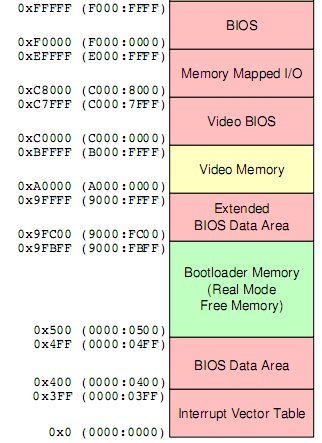
\includegraphics[width=0.5\textwidth]{../img/mmap16}
\label{fig:mmap16} 
\end{figure}

أثناء مرحلة الإقلاع وعندما يُنقل التنفيذ الى محمل النظام فان الذاكرة الرئيسية تأخذ الشكل \ref{fig:mmap16} .وأول 1024 بايت تستخدم من قبل جدول المقاطعات الذي يحوي عنوان دالة التنفيذ لكل مقاطعة للبايوس ، يليها منطقة بيانات البايوس ثم مساحة ذاكرة خالية تحوي العنوان \en{0x07c00} وهو العنوان الذي ينقل البابوس التنفيذ اليه (عنوان برنامج محمل النظام) ، ويليها منطقة بيانات بايوس الموسعة وذاكرة الفيديو والتي بمجرد الكتابة عليها تظهر الأحرف على الشاشة (\en{Memory Mapped}) ويليها البايوس على ذاكرة الفيديو ومناطق محجوزة من الذاكرة لبعض أجهزة الإدخال والإخراج ومن ثم البايوس والذي يبدأ من العنوان \en{0xf0000} وهو موجود على ذاكرة الروم (\en{Memory Mapped}) .




\section{برمجة محمل النظام}
المثال \ref{lst:useless_bootloader} يوضح أصغر محمل للنظام يمكن كتابته وتنفيذه ، باستخدام المجمع \en{NASM}\footnote{راجع الملحق \ref{apx:compile_link} لمعرفة كيفية استخدام المجمع لترجمة المحمل وكيفية نسخه الى \en{floppy disk or CD} ليتم القلاع منه سواءاً كان على جهاز فعلي أو على جهاز تخيلي (\en{Virtual Machine}) .} وهو مجمع متعدد المنصات ويوفر ميزة انتاج ملفات ثنائية \en{object code} .\\

%\lstinputlisting[language=Assembler]{./examples/ex1.asm}

\begin{english}
\fontspec[Scale=0.9]{Courier New}
\lstset{numberstyle=\tiny,numbers=left,stepnumber=1,numbersep=5pt,tabsize=2,extendedchars=true,breaklines=true,frame=b,showspaces=false, showtabs=false,xleftmargin=10pt,framexleftmargin=10pt,framexrightmargin=5pt,framexbottommargin=4pt,showstringspaces=false,language=[x86masm]Assembler}

\begin{lstlisting}[label=lst:useless_bootloader,caption=\en{Smallest Bootloader}]

;Simple Bootloader do nothing.

bits 16				; 16-bit real mode.

start:				; label are pointer.
		cli			; clear interrupt.		
		hlt			; halt the system.
		
		times	510-($-$$)	db		0		; append zeros.
		
		; $ is the address of first instruction (should be 0x07c00).
		; $$ is the address of current line.
		;  $-$$ means how many byte between start and current.
		
		; if cli and hlt take 4 byte then time directive will fill
		; 510-4 = 506 zero's.
		
		; finally the boot signature 0xaa55
		db		0x55	; first byte of a boot signature.
		db		0xaa	; second byte of a  boot signature.
		
\end{lstlisting}
\end{english}

وعندما يبدأ الجهاز بالعمل فان البايوس يقوم بنسخ هذا المحمل الى العنوان \cmd{0x0000:0x7c00} ويبدأ بتنفيذه ، وفي هذا المثال فان المحمل هذا الذي يعمل في النمط الحقيقي (\en{real mode}) لا يقوم بشيء ذو فائدة حيث يبدأ بتنفيذ الامر \cmd{cli} الذي يوقف عمل المقاطعات ، يليها الامر \cmd{hlt} الذي يوقف عمل المعالج وبالتالي يتوقف النظام عن العمل ، وبدون هذا الأمر فان المعالج سيستمر في تنفيذ أوامر لا معنى لها (\en{garbage}) والتي ستؤدي الى سقوط (\en{Crash}) النظام .  
وبسبب أن حجم المحمل يجب أن يكون \en{512} بايت وأن آخر بايتين فيه يجب أن تكونا التوقيع الخاص بالمحمل فانه يجب أن تكون أول \en{510} بايت ذات قيمة واخر بايتين هما \cmd{0xaa55} ، لذلك تم استخدام الموجه \cmd{times} لكي يتم ملئ المتبقي من أول \en{510} بايت بالقيمة صفر (ويمكن استخدام أي قيمة اخرى) وبعد ذلك تم كتابة التوقيع الخاص بالمحمل وذلك حتى يتم التعرف عليه من قِبل البايوس.

\subsection{عرض رسالة ترحيبية}
طالما ما زلنا نعمل في النمط الحقيقي فان ذلك يمكننا من استخدام مقاطعات البايوس ، وفي المثال \ref{lst:welcom_bootloader} تم  عرض رسالة باستخدام مقاطعة البايوس \cmd{int 0x10} الدالة \cmd{0xe} . 


\begin{english}
\fontspec[Scale=0.9]{Courier New}

\lstset{numberstyle=\tiny,numbers=left,stepnumber=1,numbersep=5pt,tabsize=2,extendedchars=true,breaklines=true,frame=b,showspaces=false, showtabs=false,xleftmargin=10pt,framexleftmargin=10pt,framexrightmargin=5pt,framexbottommargin=4pt,showstringspaces=false,language=[x86masm]Assembler}

\begin{lstlisting}[label=lst:welcom_bootloader,caption=\en{Welcom to OS World}]

;Hello Bootloader

bits 16				; 16-bit real mode.
org	 0x0			; this number will added to all addresses (relocating).

start:
		jmp main	; jump over data and function to entry point.


		
; ****************
;	data
; ****************

hello_msg		db		"Welcome to eqraOS, Coded by Ahmad Essam",0xa,0xd,0

; *********************************************
;	puts16: prints string using BIOS interrupt
;   input:
;				es: pointer to data segment.
;				si: point to the string
; *********************************************

puts16:
		
		lodsb			; read character from ds:si to al ,and increment si if df=0.
		
		cmp al,0		; check end of string ?
		je end_puts16	; yes jump to end.
		
		mov ah,0xe		; print character routine number.
		int 0x10		; call BIOS.
		
		jmp puts16		; continue prints until 0 is found.
		
	end_puts16:
	
		ret				
		
		
; ***************************************
;		entry point of bootloader.
; ***************************************
		
main:				

		;---------------------
		;	intit registers
		;---------------------
		
		; because bootloader are loaded at 0x07c00 we can refrence this location with many different combination of segment:offset addressing.
		
		; So we will use either 0x0000:0x7c000 or 0x:07c0:0x0000 , and in this example we use 0x07c0 for segment and 0x0 for offset.
		
		mov ax,0x07c0			
		mov ds,ax
		mov es,ax
		
		mov si,hello_msg
		call puts16

		cli			; clear interrupt.		
		hlt			; halt the system.
		
		times	510-($-$$)	db		0		; append zeros.
		
		; finally the boot signature 0xaa55
		db		0x55
		db		0xaa
		
		
\end{lstlisting}
\end{english}


%النتيجة :\\
%\missingfigure{welcome}

الشيء الملاحظ في المثال السابق هو أن مقطع الكود \en{code segment} ومقطع البيانات \en{data segment} متواجدان في نفس المكان على الذاكرة (داخل ال \en{512} بايت) لذلك يجب تعديل قيم مسجلات المقاطع للاشارة الى المكان الصحيح.
و بداية نذكر أن البايوس عندما ينقل التنفيذ الى برنامج محمل النظام الذي قمنا بكتابته فانه في حقيقة الأمر يقوم بعملية \en{far jump} والتي ينتج منها تصحيح قيم ال \cmd{cs:ip} لذلك لا داعي للقلق حول هذين المسجلين، لكن يجب تعديل قيم مسجلات المقاطع الاخرى مثل \cmd{ds,es,ss,fs,gs}. وكما نعلم أن العنوان الفيزيائي لمحمل النظام هو \cmd{0x07c00} يمكن الوصول اليه بأكثر من \en{4000} طريقة مختلفة ، لكن سوف نقتصر على استخدام العنوان \cmd{0x07c0:0x0} أو العنوان \cmd{0x0:0x7c00} نظراً لان هذه هي القيم الفعلية التي تستخدمها البايوس.

وفي حالة استخدام العنونة الاولى فان مسجلات المقاطع يجب أن تحوي القيمة \cmd{0x07c0} (كما في المثال اعلاه) أما بقية العنوانين (سواءا للمتغيرات وال \en{label}) فانها يجب أن تبدأ من القيمة \cmd{0x0}، وكما هو معروف ان المجمعات عندما تبدأ في عملية ترجمة الملف الى ملف ثنائي فانها تبدأ بترقيم العناوين بدءأ من العنوان \cmd{0x0} لذلك كانت وظيفة الموجه \cmd{org} هي عمل اعادة تعيين (\en{relocating}) للعناوين بالقيمة التي تم كتابتها ، وفي المثال أعلاه كانت القيمة هي \cmd{0x0} ، أما في حالة استخدام الطريقة الثانية للوصول الى مكان محمل النظام فان مسجلات المقاطع يجب أن تحوي القيمة \cmd{0x0} بينما المسجلات الاخرى يجب أن تبدأ قيمها من العنوان \cmd{0x7c00} ، وهذا لا يمكن بالوضع الطبيعي لان المجمعات ستبدأ من العنوان \cmd{0x0} لذلك يجب استخدام الموجه \cmd{org} وتحديد قيمة ال \en{relocate} بالقيمة \cmd{0x7c00} .



\subsection{معلومات قطاع الاقلاع}
إضافة الى محمل النظام فان قطاع الإقلاع \en{boot sector} يجب أن يحوي كذلك على معلومات تساعد في وصف نظام الملفات المستخدم ووصف القرص الذي سيتم الاقلاع منه ، هذه المعلومات تحوي معرف \en{OEM} وتحوي بيانات \en{BIOS Parameter Block} (تختصر ب \en{BPB}) ويجب أن تبدأ كل هذه البيانات من البايت رقم \en{3}\footnote{لهذا السبب فان أول تعليمة في المحمل ستكون تعليمة القفز الى الشفرة التنفيذية، وبدون القفز فان المعالج سيبدأ بتنفيذ هذه البيانات باعتبار انها تعليمات وهذا ما يؤدي في الاخر الى سقوط النظام.}. وسوف يتم استخدام هذه البيانات بكثرة أثناء تطوير محمل النظام كذلك أحد فوائد هذه البيانات هو  تعرف أنظمة التشغيل على نظام الملفات المستخدم في القرص.


\begin{english}
\fontspec[Scale=0.9]{Courier New}

\lstset{numberstyle=\tiny,numbers=left,stepnumber=1,numbersep=5pt,tabsize=2,extendedchars=true,breaklines=true,frame=b,showspaces=false, showtabs=false,xleftmargin=10pt,framexleftmargin=10pt,framexrightmargin=5pt,framexbottommargin=4pt,showstringspaces=false,language=[x86masm]Assembler}

\begin{lstlisting}[label=lst:bpb,caption=\en{Bios Parameter Block}]

OEM_ID               db        "eqraOS  "    ; Name of your OS, Must be 8 byte! no more no less.

bytes_per_sector     dw        0x200		; 512 byte per sector.
sectors_per_cluster  db        0x1          ; 1 sector per cluster.
reserved_sectors     dw        0x1          ; boot sector is reserved.
total_fats           db        0x2          ; two fats.
root_directory       dw        0xe0         ; root dir has 224 entries.
total_sectors        dw        0xb40        ; 2880 sectors in the volume.
media_descriptor     db        0xf0         ; 1.44 floppy disk.
sectors_per_fat      dw        0x9          ; 9 sector per fat.
sectors_per_track    dw        0x12         ; 18 sector per track.
number_of_heads      dw        0x2          ; 2 heads per platter.
hidden_sectors       dd        0x0          ; no hidden sector.
total_sectors_large  dd        0x0

; Extended BPB.

drive_number         db        0x0
flags                db        0x0
signature            db        0x29         ; must be 0x28 or 0x29.
volume_id            dd        0x0          ; serial number written when foramt the disk.
volume_label         db        "MOS FLOPPY " ; 11 byte.
system_id            db        "fat12   "    ;  8 byte.

\end{lstlisting}
\end{english}

%\todo[inline]{\en{explain data}}

المثال \ref{lst:bpb_bootloader} يوضح شفرة المحمل بعد اضافة بيانات \en{OEM and BPB}.


\begin{english}
\fontspec[Scale=0.9]{Courier New}

\lstset{numberstyle=\tiny,numbers=left,stepnumber=1,numbersep=5pt,tabsize=2,extendedchars=true,breaklines=true,frame=b,showspaces=false, showtabs=false,xleftmargin=10pt,framexleftmargin=10pt,framexrightmargin=5pt,framexbottommargin=4pt,showstringspaces=false,language=[x86masm]Assembler}

\begin{lstlisting}[label=lst:bpb_bootloader,caption=\en{BPB example}]

;Hello Bootloader

bits 16				; 16-bit real mode.
org	 0x0			; this number will added to all addresses (relocating).

start:
		jmp main	; jump over data and function to entry point.
		
		
;******************************************
; OEM Id and BIOS Parameter Block (BPB) 
;******************************************

; must begin at byte 3(4th byte), if not we should add nop instruction.

OEM_ID               db        "eqraOS  "    ; Name of your OS, Must be 8 byte! no more no less.

bytes_per_sector     dw        0x200		; 512 byte per sector.
sectors_per_cluster  db        0x1          ; 1 sector per cluster.
reserved_sectors     dw        0x1          ; boot sector is reserved.
total_fats           db        0x2          ; two fats.
root_directory       dw        0xe0         ; root dir has 224 entries.
total_sectors        dw        0xb40        ; 2880 sectors in the volume.
media_descriptor     db        0xf0         ; 1.44 floppy disk.
sectors_per_fat      dw        0x9          ; 9 sector per fat.
sectors_per_track    dw        0x12         ; 18 sector per track.
number_of_heads      dw        0x2          ; 2 heads per platter.
hidden_sectors       dd        0x0          ; no hidden sector.
total_sectors_large  dd        0x0

; Extended BPB.

drive_number         db        0x0
flags                db        0x0
signature            db        0x29         ; must be 0x28 or 0x29.
volume_id            dd        0x0          ; serial number written when foramt the disk.
volume_label         db        "MOS FLOPPY " ; 11 byte.
system_id            db        "fat12   "    ;  8 byte.


; ****************
;	data
; ****************

hello_msg		db		"Welcome to eqraOS, Coded by Ahmad Essam",0xa,0xd,0

; *********************************************
;	puts16: prints string using BIOS interrupt
;   input:
;				es: pointer to data segment.
;				si: point to the string
; *********************************************

puts16:
		
		lodsb			; read character from ds:si to al ,and increment si if df=0.
		
		cmp al,0		; check end of string ?
		je end_puts16	; yes jump to end.
		
		mov ah,0xe		; print character routine number.
		int 0x10		; call BIOS.
		
		jmp puts16		; continue prints until 0 is found.
		
	end_puts16:
	
		ret				
		
		
; ***************************************
;		entry point of bootloader.
; ***************************************
		
main:				

		;---------------------
		;	intit registers
		;---------------------
		
		; because bootloader are loaded at 0x07c00 we can refrence this location with many different combination
		; of segment:offset addressing.
		
		; So we will use either 0x0000:0x7c000 or 0x07c0:0x0000
		; and in this example we use 0x07c0 for segment and 0x0 for offset.
		
		mov ax,0x07c0			
		mov ds,ax
		mov es,ax
		
		mov si,hello_msg
		call puts16

		cli			; clear interrupt.		
		hlt			; halt the system.
		
		times	510-($-$$)	db		0		; append zeros.
		
		; finally the boot signature 0xaa55
		db		0x55
		db		0xaa
		

\end{lstlisting}
\end{english}


و المخرج \ref{lst:bootloader_hex} يوضح الشفرة السابقة في حالة عرضها بأي محرر سادس عشر \en{Hex Editor} حيث كما نلاحظ أن بيانات المحمل متداخلة مع الشفرة التنفيذية (تعليمات المعالج) لذلك يجب أن يتم القفز فوق هذه البيانات حتى لا تُنَفذ كتعليمات خاطئة ، كذلك يجب التأكد من آخر بايتين وأنها تحمل التوقيع الصحيح.


\begin{english}
\fontspec[Scale=0.9]{Arial}


\begin{lstlisting}[label=lst:bootloader_hex,caption=\en{Hex value of bootloader}]


Offset(h) 00 01 02 03 04 05 06 07

00000000  E9 72 00 65 71 72 61 4F  ér.eqraO
00000008  53 20 20 00 02 01 01 00  S  .....
00000010  02 E0 00 40 0B F0 09 00  .à.@.đ..
00000018  12 00 02 00 00 00 00 00  ........
00000020  00 00 00 00 00 00 29 00  ......).
00000028  00 00 00 4D 4F 53 20 46  ...MOS F
00000030  4C 4F 50 50 59 20 66 61  LOPPY fa
00000038  74 31 32 20 20 20 57 65  t12   We
00000040  6C 63 6F 6D 65 20 74 6F  lcome to
00000048  20 65 71 72 61 4F 53 2C   eqraOS,
00000050  20 43 6F 64 65 64 20 62   Coded b
00000058  79 20 41 68 6D 61 64 20  y Ahmad 
00000060  45 73 73 61 6D 0A 0D 00  Essam...
00000068  AC 3C 00 74 07 B4 0E CD  ¬<.t.´.Í
00000070  10 E9 F4 FF C3 B8 C0 07  .éôÿøÀ.
00000078  8E D8 8E C0 BE 3E 00 E8  .Ø.À¾>.è
00000080  E6 FF FA F4 00 00 00 00  æÿúô....
00000088  00 00 00 00 00 00 00 00  ........
                  ...
                  ...
000001F0  00 00 00 00 00 00 00 00  ........
000001F8  00 00 00 00 00 00 55 AA  ......Uª

\end{lstlisting}
\end{english}

ويمكن الاستفادة من هذه المحررات والتعديل المباشر في قيم الهيكس للملف الثنائي\footnote{في حالة لم نتمكن من الوصول الى ملف المصدر \en{source code}.}، فمثلا يمكن حذف التوقيع واستبداله بأي رقم ومحاولة الإقلاع من القرص ! بالتأكيد لا يمكن الاقلاع بسبب أن البايوس لن يتعرف على القرص بأنه قابل للإقلاع ، كذلك كمثال يمكن عمل حلقة لا نهائية وطباعة الجملة الترحيبة في كل تكرار ، ويجب أولا اعادة تجميع الملف الثنائي باستخدام أي من برامج ال \en{Disassembler} وإدخال تعليمة قفز بعد استدعاء دالة طباعة السلسلة الى ما قبلها.\\

\begin{english}
\fontspec[Scale=0.9]{Courier New}
\lstset{numberstyle=\tiny,numbers=left,stepnumber=1,numbersep=5pt,tabsize=2,extendedchars=true,breaklines=true,frame=b,showspaces=false, showtabs=false,xleftmargin=10pt,framexleftmargin=10pt,framexrightmargin=5pt,framexbottommargin=4pt,showstringspaces=false,language=[x86masm]Assembler}

\lstinputlisting[label=lst:bootloader_compelete,caption=\en{Complete Example}]{../examples/ch3/ex3/ex3.asm}
\end{english}

\subsection{تحميل قطاع من القرص باستخدام المقاطعة \cmd{int 0x13}}

بعد أن تم تشغيل محمل النظام لعرض رسالة ترحيبة ، فان مهمة المحمل الفعلية هي تحميل وتنفيذ المرحلة الثانية له حيث كما ذكرنا سابقا أن برمجة محمل النظام ستكون على مرحلتين وذلك بسبب القيود على حجم المرحلة الاولى ، وتكمن وظيفة المرحلة الاولى في البحث عن المرحلة الثانية من محمل النظام ونقل التنفيذ اليها ، وبعدها يأتي دور المرحلة الثانية في البحث عن نواة النظام ونقل التحكم اليها. وسنتناول الان كيفية تحميل مقطع من القرص المرن الى الذاكرة الرئيسية ونقل التحكم اليها باستخدام مقاطعة البايوس \cmd{int 0x13} .%وفي الفصل السادس سيتم دراسة الموضوع بالتفصيل عن طريق البرمجة المباشرة  لمتحكم \en{controller} القرص المرن.

\subsubsection{إعادة القرص المرن}
عند تكرار القراءة من القرص المرن فانه يجب في كل مرة أن نعيد مكان القراءة والكتابة الى أول مقطع \en{sector} في القرص وذلك لكي نضمن عدم حدوث مشاكل، وتستخدم الدالة \cmd{0x0} من المقاطعة \cmd{int 0x13} لهذا الغرض.

المدخلات :
\begin{itemize}
\item المسجل \cmd{ah}  : \cmd{0x0}.
\item المسجل \cmd{dl} : رقم محرك القرص المرن وهو \cmd{0x0}.
\end{itemize}
النتيجة:
\begin{itemize}
\item المسجل \cmd{ah} : الحالة.
\item \cmd{CF} : \cmd{0x1} اذا حدث خطأ ، \cmd{0x0} اذا تمت العملية بنجاح.

\end{itemize}

مثال:
\begin{english}
\fontspec[Scale=0.9]{Courier New}
\lstset{numberstyle=\tiny,numbers=left,stepnumber=1,numbersep=5pt,tabsize=2,extendedchars=true,breaklines=true,frame=b,showspaces=false, showtabs=false,xleftmargin=10pt,framexleftmargin=10pt,framexrightmargin=5pt,framexbottommargin=4pt,showstringspaces=false,language=[x86masm]Assembler}

\lstinputlisting[label=lst:reset_floppy_drive,caption=\en{Reset Floppy Drive}]{../examples/ch3/ex4/ex4.asm}
\end{english}

\subsubsection{قراءة المقاطع \en{sectors}}
أثناء العمل في النمط الحقيقي فاننا سنستخدم مقاطعة البايوس \cmd{int 0x13} الدالة \cmd{0x2} لقراءة المقاطع (\en{sectors}) من القرص المرن الى الذاكرة الرئيسية \en{RAM} .

المدخلات :
\begin{itemize}
\item المسجل \cmd{ah}: الدالة \cmd{0x2}
\item المسجل \cmd{al}: عدد المقاطع التي يجب قرائتها.
\item المسجل \cmd{ch}: رقم الاسطوانة  (\en{Cylinder}) ، بايت واحد.
\item المسجل \cmd{cl}: رقم المقطع ، من البت \cmd{0} - \cmd{5} ، أما اخر بتين يستخدمان مع القرص الصلب \en{hard disk}.
\item المسجل \cmd{dh}: رقم الرأس.
\item المسجل \cmd{dl} : رقم محرك القرص المرن وهو \cmd{0x0}.
\item العنوان \cmd{es:bx} : مؤشر الى المساحة التي سيتم قراءة المقاطع اليها.
\end{itemize}
النتيجة:
\begin{itemize}
\item المسجل \cmd{ah} : الحالة.
\item المسجل \cmd{al}: عدد المقاطع التي تم قرائتها.
\item \cmd{CF} : \cmd{0x1} اذا حدث خطأ ، \cmd{0x0} اذا تمت العملية بنجاح.

\end{itemize}

مثال:\\
\begin{english}
\fontspec[Scale=0.9]{Courier New}
\lstset{numberstyle=\tiny,numbers=left,stepnumber=1,numbersep=5pt,tabsize=2,extendedchars=true,breaklines=true,frame=b,showspaces=false, showtabs=false,xleftmargin=10pt,framexleftmargin=10pt,framexrightmargin=5pt,framexbottommargin=4pt,showstringspaces=false,language=[x86masm]Assembler}

\lstinputlisting[label=lst:read_floppy_disk_sector,caption=\en{Read Floppy Disk Sectors}]{../examples/ch3/ex5/ex5.asm}
\end{english}


\section{مقدمة الى نظام \en{FAT12}}
نظام الملفات هو برنامج يساعد في حفظ الملفات على القرص بحيث ينشئ لنا مفهوم الملف وخصائصه والعديد من البيانات المتعلقة به من تاريخ الانشاء والوقت ، كذلك يحتفظ بقائمة بجميع الملفات وأماكن تواجدها في القرص ، أيضاً أحد أهم فوائد أنظمة الملفات هي متابعة الأماكن الغير المستخدمة في القرص والأماكن التي تضررت بسبب أو لآخر \en{bad sectors} ، كذلك أنظمة الملفات الجيدة تقوم بعمل تجميع الملفات المبعثرة على القرص \en{Defragmentation} حتى تستفيد من المساحات الصغيرة التي ظهرت بسبب حذف ملف موجود أو تخرين ملف ذو حجم أقل من المساحة الخالية.
وبدون أنظمة الملفات فان التعامل مع القرص سيكون مستحيلا ! حيث لن نعرف ماهي المساحات الغير مستخدمة من الاخرى ولن نستطيع ان نقوم بقراءة ملف طلبه المستخدم لعرضه على الشاشة !

وبشكل عام فان نظام الملفات يتكون من:
\begin{itemize}
\item برنامج للقراءة والكتابة من القرص وسنطلق عليه اسم المحرك (\en{Driver}).
\item وجود هيكلة بيانات \en{Data Structure} معينة على القرص،يتعامل معها درايفر نظام الملفات.

\end{itemize}  

وحيث أن برمجة برنامج القراءة والكتابة تعتمد كلياُ على هيكلة نظام الملفات على القرص ، فاننا سنبدأ بالحديث عنها أولا وسوف نأخذ نظام \en{FAT12} على قرص مرن كمثال ، نظراً لبساطة هذا النظام وخلوه من التعقيدات.% وفي الفصل الخامس -بإذن الله- سيتم التطرق الى أنظمة ملفات أخرى بالتفصيل.

\subsection{قيود نظام \en{FAT12}}
يعتبر نظام \en{FAT12} من أقدم أنظمة الملفات ظهوراً وقد انتشر استخدامه في الاقراص المرنة منذ أواخر السبعينات ، ويعيب نظام \en{FAT12} :
\begin{itemize}
\item عدم دعمه للمجلدات الهرمية ويدعم فقط مجلد واحد يسمى الجذر \en{Root Directory}.
\item طول العنقود (\en{Cluster}) هو \cmd{12} بت ، بمعنى أن عدد الكلسترات هي \cmd{$2^{12}$}.
\item أسماء الملفات لا تزيد عن \cmd{12} بت.
\item يستوعب كحد أقصى \cmd{4077} ملف فقط.
\item حجم القرص يحفظ في \cmd{16} بت ، ولذا فانه لا يدعم الاقراص التي حجمها يزيد عن \cmd{32 MB}.
\item يستخدم العلامة \cmd{0x01} لتمييز التقسيمات على القرص (\en{Partitions}).


\end{itemize}

وكما ذكرنا أننا سنستخدم هذا النظام في هذه المرحلة نظراً لبساطته ، وعلى الرغم من أنه قد تلاشى استخدامه في هذا الزمن الا انه يعتبر أساس جيد للأنظمة المتقدمة لذا وجب دراسته.


\subsection{هيكلة نظام \en{FAT12} على القرص}
عند تهئية القرص المرن\footnote{سواءاً كانت التهئية من قبل درايفر نظام الملفات الذي سنقوم ببرمجته أو كانت من قبل نظام الشتغيل المستخدم أثناء عملية التطوير ، فمثلا في ويندوز يمكن إعادة تهئية القرص المرن بنظام \en{FAT12} .} (\en{Format}) بنظام \en{FAT12} فان تركيبة القرص تكون على الشكل \ref{fig:fat12structure} :\\
%\missingfigure{fat12structure}
\begin{figure}[h!] 
  \caption{هيكلة نظام \en{FAT12} على القرص}
  \centering
   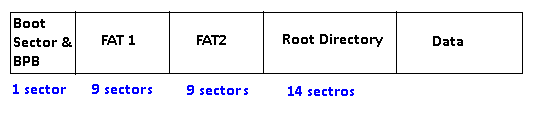
\includegraphics[width=0.7\textwidth]{../img/fat12}
 \label{fig:fat12structure} 
\end{figure}

وأول مقطع هو مقطع الاقلاع (\en{Boot Sector}) ويحوي شفرة محمل النظام (المرحلة الاولى) بالاضافة الى بيانات ومعلومات \en{BPB and OEM id} ، هذا المقطع عنوانه الفيزيائي على القرص هو : المقطع \cmd{1} المسار \cmd{0} الرأس \cmd{0} وهذا العنوان هو الذي يجب تمرير الى مقاطعة البايوس \cmd{int 0x13} التي تقوم بالقراءة من القرص كذلك في حالة ما أردنا التعامل المباشر مع متحكم القرص المرن.
ونظرً لصعوبة هذه العنونة والتي تعرف ب \en{Absolute Sector} فان أنظمة الملفات تتعامل مع نظام عنونة مختلف للوصول الى محتويات القرص ، فبدلاً من ذكر كل من المقطع والمسار والرأس للوصول الى مقطع ما فان هذه العنونة تستخدم فقط رقم للمقطع .
نظام العنونة الذي تستخدمه أنظمة الملفات يسمى بالعنونة المنطقية (\en{Logical Sector Addressing}) ويختصر ب \en{LBA} هو نظام بسيط يعتمد على ترقيم المقاطع بشكل متسلسل بدئاً من مقطع الاقلاع (\en{Boot Sector}) والذي يأخذ العنوان \cmd{0} ، والمقطع الثاني \cmd{1} وهكذا هلم جرا حتى نصل الى آخر مقطع في القرص. وبما أنه يجب استخدام العنونة الحقيقة بدلا من المنطقية لحظة القراءة من القرص (تذكر مقاطعة البايوس \cmd{int 0x13} والمسجلات التي يجب ادخال قيمها) فانه يجب ايجاد طريقة للتحويل من العنونة الحقيقة الى المنطقية -سنناقش الموضوع لاحقا-.
ننتقل الى المقطع التالي لمقطع الإقلاع وهو مقطع (أو عدة مقاطع) يمكن أن يحجزها المبرمج لاداء أي وظيفة يريدها وتسمى المقاطع المحجوزة الاضافية \en{Extra Reserved Sectors} ، والمقصود بمحجوزة أي انه لا يوجد لها وجود في دليل \en{FAT} ، ومقطع الإقلاع هو مقطع محجوز دائما لذلك كانت قيمة المتغير  \en{reserved sectors} في معلومات \en{BPB} هي واحد ، وفي حالة ما أردت حجز مقاطع أخرى كل ما عليك هو زيادة هذه القيمة بعدد المقاطع المرغوبة ، وللوصول الى محتويات هذا المقطع الاضافي(ان كان له وجود) فان العنوان الحقيقي له هو المقطع \en{2} المسار \en{0} الرأس \en{0} ، أما العنوان المنطقي له هو المقطع \en{1}. وبشكل عام فانه في الغالب لا يتم استخدام مقاطع اضافية سوى مقطع الاقلاع .
المقطع الثالث هو جدول \en{FAT} ، وهو جدول يحوي سجلات بطول \cmd{12} بت عن كل كلستر (\en{Cluster}) في القرص ، بيانات هذا السجل توضح ما اذا كان الكلستر قيد الاستخدام أم لا ، وهل هو آخر كلستر للملف أم لا وإذا كان ليس باخر فانه يوضح لنا الكلستر التالي للملف ، ويوضح الشكل التالي تركيبة هذا الجدول\\
%\missingfigure{fat}

اذاً هذا وظيفة هذا الجدول هي معرفة الكلسترات الخالية من غيرها كذلك الوظيفة الاخرى هي معرفة جميع الكلسترات لملف ما ويتم ذلك بالنظر الى قيمة السجل (قيمة ال \cmd{12} بت) ، والقيم هي :

\begin{itemize}
\item القيمة \cmd{0x00}: تدل على أن الكلستر خالي.
\item القيمة \cmd{0x01} : تدل على أن الكلستر محجوز.
\item القيم من \cmd{0x02} الى \cmd{0xfef} : تدل على عنوان الكلستر التالي (بمعنى آخر أن الكلستر محجوز وتوجد كلسترات متبقية للملف).
\item القيم من \cmd{0xff0} الى \cmd{0xff6}: قيم محجوزة.
\item القيمة \cmd{0xff6} : تدل على \en{Bad Cluster}.
\item القيم من \cmd{0xff8} الى \cmd{0xfff}: تدل على أن هذا الكلستر هو الاخير للملف. 

\end{itemize}

ويمكن النظر الى جدول \en{FAT} بأنه مصفوفة من القيم أعلاه ، وعندما نريد تحميل ملف فاننا سنأتي بعنوان أول كلستر له من جدول \en{Root Directory} (سنأتي عليها لاحقا) وبعدها نستخدم عنوان الكلستر ك \en{index} الى جدول \en{FAT} ونقرأ القيمة المقابله للكلستر ، فاذا كانت القيمة بين \cmd{0x02} الى \cmd{0xfef} فانها تدل على الكلستر التالي للملف ، ومن ثم سنستخدم هذه القيمة أيضا ك \en{index} ونقرأ القيمة الجديدة ، ونستمر على هذا الحال الى أن نقرأ قيمة تدل على نهاية الملف.
هذا الجدول \en{FAT} يبدأ من المقطع المنطقي \cmd{1}\footnote{بافتراض الوضع الغالب وهو عدم وجود مقاطع إضافية باستثناء مقطع الإقلاع} وطوله \cmd{9} مقاطع أي أن نهاية هذا الجدول تكون في المقطع تكون في آخر المقطع \cmd{10}، ولمعرفة العنوان الحقيقي للمقطع فانه يمكن استخدام بعض المعادلات للتحويل ، والقسم التالي سيوضح ذلك بالاضافة الى شرح مبسط عن هيكلة القرص المرن وكيفية حفظه للبيانات .
وبعد جدول \en{FAT} توجد نسخة أخرى من هذا الجدول وتستخدم كنسخة احتياطية \en{backup} وهي بنفس حجم وخصائص النسخة الاولى ، وبعدها يأتي دليل الجذر \en{Root Directory} وهو مصفوفة من \cmd{224} سجل كل سجل بطول \cmd{32} بايت ، وظيفية هذا الدليل هي حفظ أسماء الملفات الموجودة على القرص المرن بالاضافة الى العديد من المعلومات التي تخص وقت الانشاء والتعديل وحجم الملف وعنوان أول كلستر للملف ، عنوان الكلستر هو أهم معلومة لكي نستطيع تحميل الملف كاملا ، حيث كما ذكرنا أن هذا العنوان سيعمل ك \en{index} في جدول \en{FAT} وبعدها سنحدد ما اذا كانت توجد كلسترات أخرى يجب تحميلها أم أن الملف يتكون من كلستر واحد. والجدول التالي يوضح محتويات السجل الواحد في دليل ال \en{root directory} بداءاً من البايت الاول الى الاخير:

\begin{itemize}

\item البايتات \cmd{0}-\cmd{7}: اسم الملف( وفي حالة كان الحجم أقل من \cmd{8} بايت يجب استخدام حرف المسافة لتعبئة المتبقي).
\item البايتات \cmd{8}-\cmd{10}: امتداد الملف(يجب استخدام المسافة أيضا لتعبئة المتبقي).
\item البايت \cmd{11}: خصائص الملف وهي :
\begin{itemize}
\item البت \cmd{0}: القراءة فقط.
\item البت \cmd{1}: مخفي.
\item البت \cmd{2}: ملف نظام.
\item البت\cmd{3}: اسم القرص \en{Volume Label}.
\item البت \cmd{4}: الملف هو مجلد فرعي.
\item البت \cmd{5}: أرشيف.
\item البت \cmd{6}: جهاز.
\item البت \cmd{7}: غير مستخدم.
\end{itemize}

\item البايت \cmd{12}: غير مستخدم.
\item البايت \cmd{13}: وقت الانشاء بوحدة \en{MS}.
\item البايتات \cmd{14}-\cmd{15}: وقت الانشاء بالترتيب التالي:

\begin{itemize}
\item البتات \cmd{0}-\cmd{4}: الثواني (\cmd{0}-\cmd{29}).
\item البتات \cmd{5}-\cmd{10}: الدقائق (\cmd{0}-\cmd{59}).
\item البتات \cmd{11}-\cmd{15}: الساعات (\cmd{0}-\cmd{23}).
\end{itemize}

\item البايتات \cmd{16}-\cmd{17}: سنة الانشاء بالترتيب التالي:

\begin{itemize}
\item البتات \cmd{0}-\cmd{4}: السنة (\cmd{0}=\cmd{1980}; \cmd{127}=\cmd{2107}).
\item البتات \cmd{5}-\cmd{8}: الشهر (\cmd{1}=يناير; \cmd{12}=ديسمبر).
\item البتات \cmd{9}-\cmd{15}: الساعة (\cmd{0}-\cmd{23}).
\end{itemize}

\item البايتات \cmd{18}-\cmd{19}: تاريخ آخر استخدام (تتبع نفس الترتيب السابق).
\item البايتات \cmd{20}-\cmd{21}: \en{EA index}.
\item البايتات \cmd{22}-\cmd{23}: وقت آخر تعديل (تتبع نفس ترتيب البايتات \cmd{14}-\cmd{15}).
\item البايتات \cmd{24}-\cmd{25}: تاريخ آخر تعديل (تتبع نفس ترتيب البايتات \cmd{16}-\cmd{17}).
\item البايتات \cmd{26}-\cmd{27}: عنوان أول كلستر للملف.
\item البايتات \cmd{28}-\cmd{29}: حجم الملف.


\end{itemize}

ويجب ملاحظة أن حجم السجلات هو ثابت \en{Fixed Lenght Record} فمثلا اسم الملف يجب ان يكون بطول \cmd{8} بايت وفي حالة زاد على ذلك فان هذا سوف يحدث ضرراً على هذا الدليل ، أيضا في حالة كان الاسم بحجم أقل من المطلوب فانه يجب تكلمة العدد الناقص من الحروف بحرف المسافة \en{Space}.

\subsection{هيكلة القرص المرن}
يتكون القرص المرن من قرص \en{Platter} (أو عدة أقراص) مقسمة الى مسارات (\en{Tracks}) وكل من هذه المسارات يتكون من العديد من القطاعات ويوجد عادة رأسين للقراءة والكتابة على كل قرص. وفي الاقراص المرنة ذات الحجم \cmd{1.44 MB} يوجد \cmd{80} مساراً (من المسار \cmd{0} الى المسار \cmd{79}) وكل مسار يتكون من \cmd{18} قطاع ، وبالتالي فان عدد القطاعات الكلية هي \en{$80*18*2$} وتساوي \cmd{2880} قطاعاً.

ولتخزين بيانات على القرص فانه يجب تحديد العنوان الحقيقي والذي يتكون من عنوان القطاع والمسار والرأس ، وأول قطاع في القرص (قطاع الاقلاع) يأخذ العنوان: القطاع \cmd{1} المسار \cmd{0} الرأس \cmd{0} ، والقطاع الثاني يأخذ العنوان: القطاع \cmd{2} المسار \cmd{0} الرأس \cmd{0} ، وهكذا يستمر نظام التخزين في القرص المرن الى أن يصل الى العنوان \cmd{18} المسار \cmd{0} الرأس \cmd{0} وهو عنوان آخر قطاع على المسار الاول والرأس الاول ، وسيتم حفظ البيانات التالية في الرأس الثاني على العنوان: القطاع \cmd{1} المسار \cmd{0} الرأس \cmd{1} ويستمر الى أن يصل الى آخر قطاع في هذا المسار على الرأس الثاني، وبعدها سيتم حفظ البيانات التالية في الرأس الاول المسار الثاني ... ،وهكذا. %والصورة التالية توضح شكل القرص المرن بعد عمل تهئية (\en{Format}) له.\\
%\missingfigure{floppyforamtted}

\subsection{القراءة و الكتابة من نظام \en{FAT12} }
حتى نتمكن من التعامل مع القرص المرن (قراءة وكتابة القطاعات) فانه يلزمنا برمجة درايفر  لنظام \en{FAT12} والذي سيعمل كوسيط بين المستخدم وبين القرص المرن، بمعنى أن أي طلب لقراءة ملف ما يجب أن تذهب أولا الى نظام \en{FAT12} حيث سيقرر ما اذا كان الملف موجوداً أم لا (عن طريق البحث في دليل \en{Root directory}) وفي حالة كان موجوداً سيعود لنا بجميع خصائص الملف ورقم أول كلستر له لكي نتمكن من تحميل الملف كاملاً ، ونفس المبدأ في حالة طلب المستخدم كتابة ملف على القرص فان درايفر نظام \en{FAT12} سيبحث في جدول \en{FAT} عن مساحة خالية مناسبة للملف وذلك باتباع أحد الخورازميات المعروفة وبعدها سيتم حفظ الملف وكتابة البيانات المتعلقة به في دليل \en{Root directory} .

وسنأخذ مثال على الموضوع وذلك ببرمجة المرحلة الثانية من محمل النظام \en{Second Stage Bootloader} وستقتصر وظيفته حالياً في طباعة رسالة ترحيبة دلالة على أنه تم تحميل وتنفيذ المرحلة الثانية بنجاح ، وفي الأقسام التالية سنبدأ في تطوير المرحلة الثانية وتجهيز مرحلة الانتقال الى بيئة \cmd{32} بت.

مهمة المرحلة الاولى ستتغير عن ما سبق ، حيث الان يجب على المرحلة الاولى أن تقوم بالبحث عن المرحلة الثانية من محمل النظام ونقل التنفيذ اليها ، ويتم هذا وفق الخطوات التالية:

\begin{enumerate}
\item تحميل جدول \en{Root Directory} من القرص الى الذاكرة ومن ثم البحث عن ملف المرحلة الثانية وأخذ رقم أول كلستر له.

\item تحميل جدول \en{FAT} من القرص الى الذاكرة ومن ثم تحميل جميع الكلسترات للملف.

\item نقل التنفيذ الى أول بايت في المرحلة الثانية من محمل النظام.
\end{enumerate}

\subsubsection{إنشاء المرحلة الثانية من محمل النظام}

بداية سنقوم بإنشاء المرحلة الثانية من محمل النظام ونسخها الى القرص المرن ، ونظراً لان تطوير نظامنا الخاص يجب ان يتم تحت نظام آخر فان هذا النظام الآخر غالبا ما يحوي درايفر لنظام ملفات \en{FAT12} حيث يتكفل بعملية كتابة البيانات الى جدول \en{Root Directory} بالاضافة الى البحث عن كلسترات خالية في جدول \en{FAT} دون أي تدخل من قبل مطور النظام الجديد، لذلك في هذه المرحلة من التطوير سنتجاهل جزئية الكتابة في نظام \en{FAT12} ونترك المهمة لنظام التشغيل الذي نعتمد عليه في عملية تطوير النظام الجديد ، وبهذا سيكون الدرايفر الذي سننشئه في هذا الفصل ما هو الا جزء من الدرايفر الكامل الذي سيتم تكلمته لاحقا بمشيئة الله.والشفرة التالية توضح مثال للمرحلة الثانية من المحمل لعرض رسالة بسيطة.

\begin{english}
\fontspec[Scale=0.9]{Courier New}
\lstset{numberstyle=\tiny,numbers=left,stepnumber=1,numbersep=5pt,tabsize=2,extendedchars=true,breaklines=true,frame=b,showspaces=false, showtabs=false,xleftmargin=10pt,framexleftmargin=10pt,framexrightmargin=5pt,framexbottommargin=4pt,showstringspaces=false,language=[x86masm]Assembler}

\lstinputlisting[label=lst:hello_stage2,caption=\en{Hello Stage2}]{../examples/ch3/ex6/stage2.asm}
\end{english}

وسيتم تسمية الملف بالاسم \en{stage2.asm} أما الملف الناتج من عملية التجميع سيكون بالاسم \en{stage2.sys} ويمكن تسميته بأي اسم اخر بشرط أن لا يزيد الاسم عن \cmd{8} حروف والامتداد عن \cmd{3} حروف ، وفي حالة كان طول الاسم أقل فان درايفر \en{FAT12} سيقوم باضافة مسافات \en{Spaces} حتى لا يتضرر جدول \en{Root Directory}. ويمكننا أن نفرق بين اسماء الملفات الداخلية (وهي التي يتم اضافة مسافات عليها ويستخدمها نظام \en{FAT12}) والأسماء الخارجية (وهي التي ينشئها المستخدم).

\subsubsection{تحميل ال \en{Root Directory} الى الذاكرة}
جدول \en{Root Directory} يحوي أسماء كل الملفات و أماكن تواجدها على القرص لذا يجب تحميله أولا والبحث عن ملف المرحلة الثانية (ذو الاسم الخارجي \en{stage2.sys}) وعند البحث يجب البحث بالاسم الداخلي الذي يستخدمه نظام الملفات لذلك يجب أن نبحث عن الملف \en{"stage2  sys"} ، ونأتي برقم الكلستر الأول للملف.

وقبل تحميل هذا الجدول فانه يجب علينا أولاً معرفة عنوان أول قطاع فيه وحساب عدد القطاعات التي يشغلها هذا الجدول ، كذلك يجب تحديد المساحة الخالية (\en{Buffer}) لكي يتم نقل هذا الجدول اليها. والشفرة التالية توضح كيفية عمل ذلك.
 
\begin{english}
\fontspec[Scale=0.9]{Courier New}
\lstset{numberstyle=\tiny,numbers=left,stepnumber=1,numbersep=5pt,tabsize=2,extendedchars=true,breaklines=true,frame=b,showspaces=false, showtabs=false,xleftmargin=10pt,framexleftmargin=10pt,framexrightmargin=5pt,framexbottommargin=4pt,showstringspaces=false,language=[x86masm]Assembler}

\lstinputlisting[label=lst:load_root_dir,caption=\en{Load Root directory}]{../examples/ch3/ex7/ex7.asm}
\end{english}

بعد تحميل هذا الجدول يجب البحث فيه عن اسم ملف المرحلة الثانية من محمل النظام ومن ثم حفظ رقم أول كلستر له في حالة كان الملف موجوداً ، أما اذا كان الملف غير موجود فنصدر رسالة خطأ ونوقف النظام عن العمل. والشفرة التالية توضح ذلك.

\begin{english}
\fontspec[Scale=0.9]{Courier New}
\lstset{numberstyle=\tiny,numbers=left,stepnumber=1,numbersep=5pt,tabsize=2,extendedchars=true,breaklines=true,frame=b,showspaces=false, showtabs=false,xleftmargin=10pt,framexleftmargin=10pt,framexrightmargin=5pt,framexbottommargin=4pt,showstringspaces=false,language=[x86masm]Assembler}

\lstinputlisting[label=lst:find_stage2,caption=\en{Find Stage2 Bootloader}]{../examples/ch3/ex8/ex8.asm}
\end{english}

\subsubsection{تحميل جدول \en{FAT} الى الذاكرة}
جدول \en{FAT} يوضح حالة كل الكلسترات الموجودة على القرص سواءا كانت خالية أم معطوبة أم انها مستخدمة ، ويجب تحميل هذا الجدول الى الذاكرة لكي نستطيع عن طريق رقم الكلستر الذي تحصلنا عليه من جدول \en{Root Directory} أن نحمل جميع كلسترات الملف.
وبنفس الطريقة التي قمنا بها لتحميل جدول \en{Root Directory} سيتم بها تحميل جدول \en{FAT} حيث يجب تحدد عنوان أول قطاع للجدول و عدد القطاعات التي يشغلها الجدول ، وكذلك المساحة الخالية في الذاكرة لكي يتم حفظ الحدول بها . والشفرة التالية توضح ذلك.

\begin{english}
\fontspec[Scale=0.9]{Courier New}
\lstset{numberstyle=\tiny,numbers=left,stepnumber=1,numbersep=5pt,tabsize=2,extendedchars=true,breaklines=true,frame=b,showspaces=false, showtabs=false,xleftmargin=10pt,framexleftmargin=10pt,framexrightmargin=5pt,framexbottommargin=4pt,showstringspaces=false,language=[x86masm]Assembler}

\lstinputlisting[label=lst:load_fat,caption=\en{Load FAT Table}]{../examples/ch3/ex9/ex9.asm}
\end{english}

\subsubsection{تحميل كلسترات الملف}
وحدة القراءة والكتابة للقرص المرن هي بالقطاع \en{Sector} لكن نظام الملفات \en{FAT12} يتعامل مع مجموعة من القطاعات ككتلة واحدة \en{Cluster}، وكلما كبر حجم الكلستر زادت المساحات الخالية بداخله \en{Internel Fragmentation} لذلك يجب اختيار حجم ملائم ، وفي تنفيذ نظام \en{FAT12} على قرص مرن أخترنا أن كل كلستر يقابل قطاع واحد فقط من القرص المرن.
المشكلة التي ستواجهنا هي كيفية قراءة كلستر من القرص ، فالقرص المرن لا يقرأ اي قطاع الا بتحديد العنوان المطلق له \en{Absolute Address} ولذلك يجب تحويل رقم الكلستر الى عنوان مطلق وتحويل عنوان \en{LBA} أيضا الى عنوان مطلق.

التحويل من رقم \en{Cluster} الى عنوان \en{LBA} يتم كالاتي:

\begin{english}
\fontspec[Scale=0.9]{Courier New}
\lstset{numberstyle=\tiny,numbers=left,stepnumber=1,numbersep=5pt,tabsize=2,extendedchars=true,breaklines=true,frame=b,showspaces=false, showtabs=false,xleftmargin=10pt,framexleftmargin=10pt,framexrightmargin=5pt,framexbottommargin=4pt,showstringspaces=false,language=[x86masm]Assembler}

\lstinputlisting[label=lst:cluster_to_lba,caption=\en{Convert Cluster number to LBA}]{../examples/ch3/ex10/ex10.asm}
\end{english}


حيث يتم طرح العدد \cmd{2} من رقم الكلستر وهذا بسبب أن أول رقم كلستر في نظام \en{FAT12} هو \cmd{2} - كما سنرى ذلك لاحقا-.

وللتحويل من عنوان \en{LBA} الى عنوان \en{Absolute Address} :

\begin{english}
\fontspec[Scale=0.9]{Courier New}
\lstset{numberstyle=\tiny,numbers=left,stepnumber=1,numbersep=5pt,tabsize=2,extendedchars=true,breaklines=true,frame=b,showspaces=false, showtabs=false,xleftmargin=10pt,framexleftmargin=10pt,framexrightmargin=5pt,framexbottommargin=4pt,showstringspaces=false,language=[x86masm]Assembler}

\lstinputlisting[label=lst:lba_to_cluster,caption=\en{Convert LBA to CHS}]{../examples/ch3/ex11/ex11.asm}
\end{english}

ولتحميل كلستر من القرص يجب أولا الحصول على رقمه من جدول \en{Root Directory} وبعد ذلك نقوم بتحويل هذا الرقم الى عنوان \en{LBA} وبعدها نقوم بتحويل عنوان \en{LBA} الى عنوان مطلق \en{Abolsute Address} ومن ثم استخدام مقاطعة البايوس \cmd{int 0x13} لقراءة القطاعات من القرص، والشفرة التالية توضح ذلك.

\begin{english}
\fontspec[Scale=0.9]{Courier New}
\lstset{numberstyle=\tiny,numbers=left,stepnumber=1,numbersep=5pt,tabsize=2,extendedchars=true,breaklines=true,frame=b,showspaces=false, showtabs=false,xleftmargin=10pt,framexleftmargin=10pt,framexrightmargin=5pt,framexbottommargin=4pt,showstringspaces=false,language=[x86masm]Assembler}

\lstinputlisting[label=lst:load_cluster,caption=\en{Load Cluster}]{../examples/ch3/ex12/ex12.asm}
\end{english}

ودالة قراءة القطاعات من القرص تستخدم مقاطعة البايوس \cmd{int 0x13} وهي تعمل فقط في النمط الحقيقي ويجب استبدالها لاحقا عند التحويل الى النمط المحمي بدالة اخرى \cmd{32-bit}.

\begin{english}
\fontspec[Scale=0.9]{Courier New}
\lstset{numberstyle=\tiny,numbers=left,stepnumber=1,numbersep=5pt,tabsize=2,extendedchars=true,breaklines=true,frame=b,showspaces=false, showtabs=false,xleftmargin=10pt,framexleftmargin=10pt,framexrightmargin=5pt,framexbottommargin=4pt,showstringspaces=false,language=[x86masm]Assembler}

\lstinputlisting[label=lst:read_sector_routine,caption=\en{Read Sectors Routine}]{../examples/ch3/ex13/ex13.asm}
\end{english}

ولتحميل بقية كلسترات الملف يجب أخذ رقم أول كلستر للملف والذهاب به الى جدول \en{FAT} وقراءة القيمة المقابلة له والتي ستدل على ما اذا كان هذا آخر كلستر أم أن هنالك كلسترات اخرى يجب تحميلها.ويلزم الأخذ بالاعتبار بنية جدول \en{FAT} وانه يتكون من سجلات بطول \cmd{12} بت وتعادل بايت ونصف ، أي أنه اذا كان رقم الكلستر هو \cmd{0} فاننا يجب أن نقرأ السجل الاول من جدول \en{FAT} وبسبب انه لا يمكن قراءة \cmd{12} بت فسوف تتم قراءة \cmd{16} بت (السجل الاول بالاضافة الى نصف السجل الثاني) وعمل \en{mask} لاخر \cmd{4} بت (لازالة ما تم قرائته من السجل الثاني). وفي حالة كان رقم الكلستر هو  \cmd{1} فيجب قراءة السجل الثاني من جدول \en{FAT} والذي يبدأ من البت \cmd{12}-\cmd{23} وبسبب أنه لا يمكن قراءة \cmd{12} بت سنقوم بقراءة \cmd{16} بت أي من البت \cmd{8}-\cmd{23} وازالة أول \cmd{4} بت.\\

وباختصار، لقراءة القيمة المقابلة لرقم كلستر ما فيجب أولا تطبيق القانون :\\
\begin{english}
\en{$cluster=cluster+(cluster/2)$}\\
\end{english}

 وقراءة \cmd{16} بت ، وفي حالة ما اذا كان رقم الكلستر هو رقم زوجي فيجب عمل \en{Mask} لاخر \cmd{4} بت ، أما اذا كان رقم الكلستر فردي فيجب ازالة أول \cmd{4} بت . والشفرة التالية توضح كيفية تحميل جميع كلسترات المرحلة الثانية من محمل النظام الى الذاكرة ونقل التنفيذ اليها .

\begin{english}
\fontspec[Scale=0.9]{Courier New}
\lstset{numberstyle=\tiny,numbers=left,stepnumber=1,numbersep=5pt,tabsize=2,extendedchars=true,breaklines=true,frame=b,showspaces=false, showtabs=false,xleftmargin=10pt,framexleftmargin=10pt,framexrightmargin=5pt,framexbottommargin=4pt,showstringspaces=false,language=[x86masm]Assembler}

\lstinputlisting[label=lst:read_fat_entry,caption=\en{Read FAT entry}]{../examples/ch3/ex14/ex14.asm}
\end{english}

\end{document}